\chapter{Metodologia}
\section{Detalhes Técnicos}
\label{sec:tech}

A nossa aplicação foi criada a caráter informativo, com textos e elementos visuais atrativos, onde foi desenvolvida inteiramente utilizando frameworks Next.js. Logo, por ser uma interface com estruturas lógicas, não possui a nescessidade da construção de uma configuração de back-end, visto que não haverá nenhum dado externo armazenado. Portanto, o usuário poderá navegar pela plataforma sem precisar fazer cadastro, login ou fazer a inserção de qualquer outro tipo de dado.

\subsection{Front-End}
O Front-end é implementado em \cite{Next.Js} como mostra a Figura \ref{fig:logicFront}

\begin{figure}[h!]
    \centering
    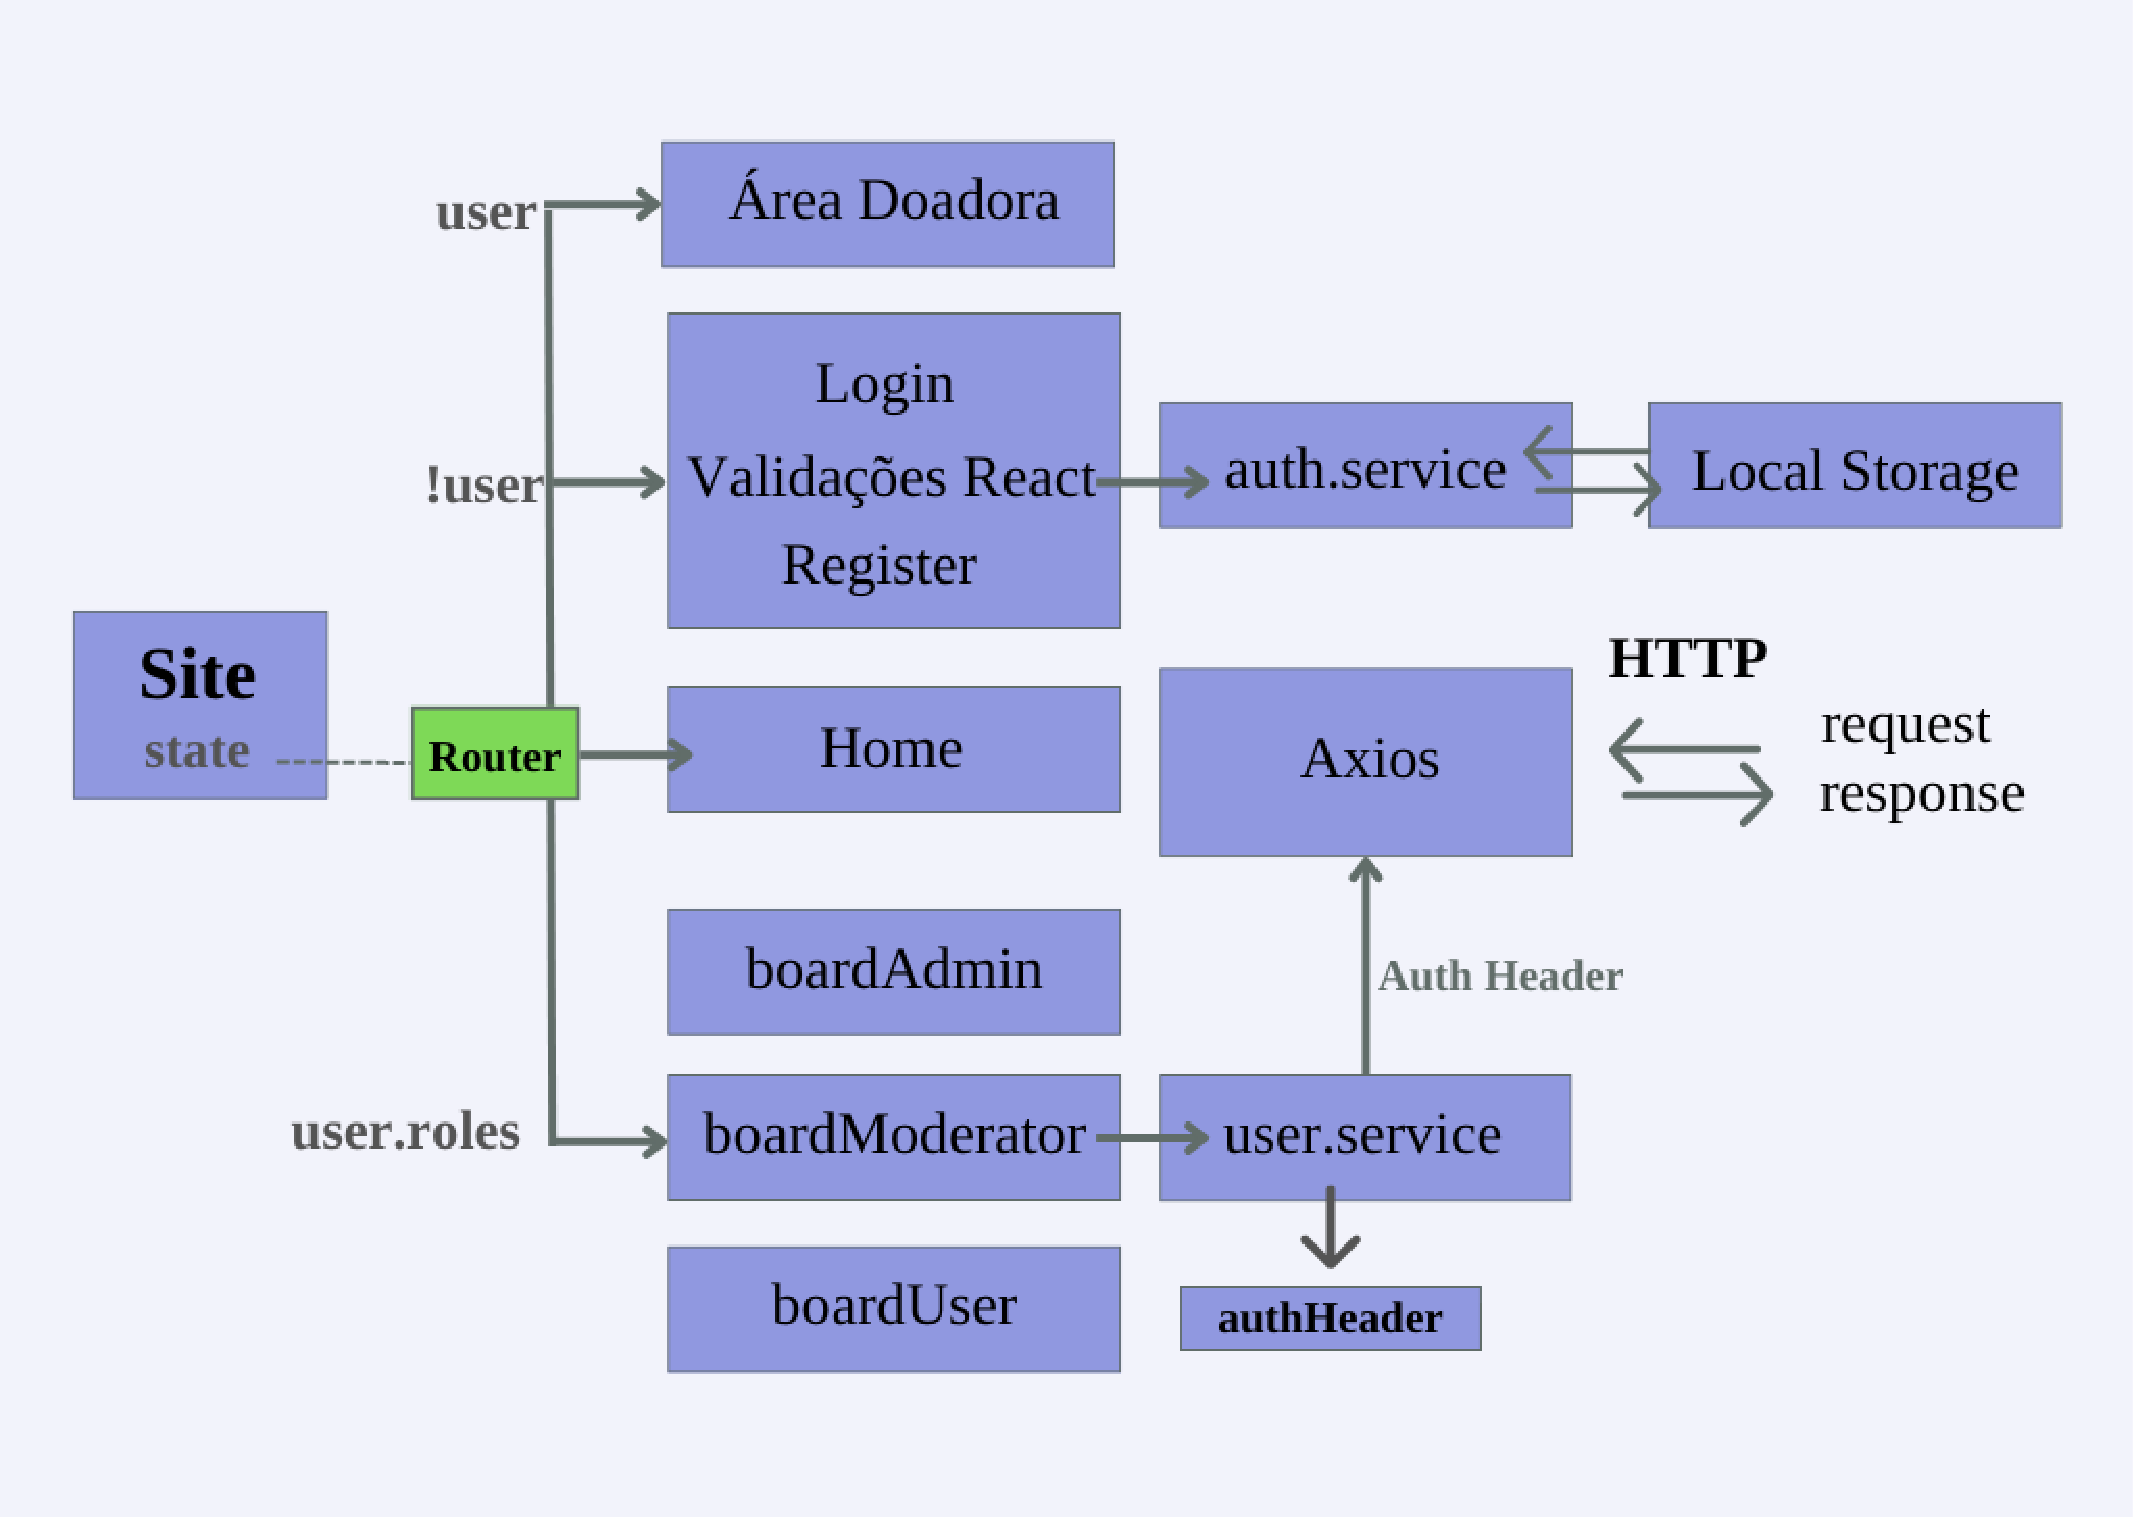
\includegraphics[width=1.0\textwidth]{Figuras/Frontpdf.pdf}
    \caption{Estrutura lógica do Front-End composta por React}
    \label{fig:logicFront}
\end{figure}

A plataforma apresenta uma tela inicial onde exibe o material de apoio para introduzir o conteúdo para estudo e aprendizado. Nesta tela também é apresentado um botão de denuncia, de extrema importância para o acionamento imediato do suporte nescessário par a situação. E a área também dispões de uma barra de navegação lateral que aponta os componentes a seguir:

\begin{itemize}


    \item Área do questionário, onde o usuário vai poder fazer a interação gameficada baseado no conteúdo apresentado na plataforma. O quiz apresenta três níveis: fácil, médio e dificil, desta forma o usuário irá fixar melhor o conteúdo apresentado na plataforma. 
 
    \item  Área de certificação, após a conclusão do quiz, o usuário poderá receber o certificado de acordo com a quantidade de acertos. Para receber o certificado o aluno precisa acertar mais de 7 questões. Criamos um algoritmo de verificação onde foram setadas as dificuldades em uma variável, em seguida adiocionamos uma codição no código que análisa a quantidade de acertos no quiz. 
    Caso o usuário não atinja a pontuação necessária, ele será direcionado para uma página onde será dado a opção de poder tentar realizar o quiz novamente. 
    

    \item Na área de indicações e materiais de estudo o usuário vai encontrar links de podcasts, sites, documentos literários e alguns materiais de estudo para o aprofundamento no conteúdo.
    
    \item Área de saiba mais que faz uma apresentação um pouco mais profunda de todo o contexto trazendo um pouco da história da empresa Placamãe.org, surgimento, trajetório e quais os impactos dentro da sociedade.
   
   
\end{itemize}

\clearpage

\subsubsection{Back-End}
Nossa plataforma tem caráter informativo, então, não se faz nescessário utilizar um sistema back-end pois não existe tráfego de dados. 



\begin{itemize}
 
\end{itemize}



\chapter{Requisitos funcionais e não funcionais}
\section{Requisitos Funcionais:}
\begin{itemize}
  \item O site permite a navegação entre as seções mencionadas no menu.
  \item  Os quizzes são divididos em categorias de dificuldade (fácil, média e difícil).
  \item O site fornece materiais de estudo relacionados aos quizzes.
   \item Home é o componente público de acesso a todos os usuários.
   \item Há uma funcionalidade de denúncia acessível em todo o site.
   \item O site exibe recomendações de livros, podcasts e artigos científicos sobre ciberbullying.
   \item  Links para redes sociais são funcionais onde direcionam para as páginas corretas.
\item Há um e-mail de contato visível em todo o site.
\item Informações sobre consultoria, palestras e cursos estão disponíveis.
\end{itemize}

\label{sec:tech}


\subsection{Requisitos Não Funcionais:}
\begin{itemize}
\item O site é seguro, utilizando protocolos HTTPS.
\item O site é acessível, seguindo as diretrizes WCAG. 
\item O site está esponsivo para dispositivos móveis e que suas fontes de informações são verificadas e de uso comprovado academicamente
\end{itemize}
\clearpage

\section{Descrição Geral}
\label{sec:descricao}
Para o projeto final, foi proposto o desafio de desenvolver um site interativo, enriquecido com um jogo, com o objetivo de ser educativo, envolvente e um canal para denúncias. Este site tem como meta auxiliar professores, alunos e famílias a compreenderem e combaterem o cyberbullying, alertando sobre os riscos e as ações que podem levar a incidentes de bullying. \\

O cyberbullying é um problema crescente na era digital, com consequências potencialmente devastadoras para os indivíduos afetados. Através deste projeto, espera-se fornecer uma ferramenta valiosa para combater este problema, educando e informando os usuários sobre o cyberbullying e fornecendo um meio seguro e anônimo para denunciar incidentes de bullying.\\

Este projeto está alinhado à Agenda 2030 da ONU, que estabelece 16 Objetivos de Desenvolvimento Sustentável (ODS). Em particular, o projeto se concentra no ODS 3, que é voltado para a saúde e o bem-estar. Este objetivo enfatiza a importância de garantir vidas saudáveis e promover o bem-estar para todos, em todas as idades. Ao combater o cyberbullying, este projeto contribui para este objetivo, ajudando a criar um ambiente online mais seguro e saudável para todos.\\

A plataforma foi projetada para facilitar todos os passos que envolvem esse processo, além de oferecer funcionalidades que visam incentivar o engajamento de novos indivíduos na luta contra o cyberbullying. A plataforma online será dividida em quatro seções principais, cada uma com suas próprias funcionalidades, que serão descritas a seguir.

\begin{itemize}
    \item A seção "Questionário" apresentará perguntas de níveis fácil, médio e difícil sobre o tema, baseadas em ebooks, podcasts e artigos científicos. Esta seção também incluirá exemplos práticos de situações de cyberbullying no dia a dia, com um total de 13 questões para cada nível. O objetivo desta seção é testar o conhecimento do usuário sobre o tema.

    \item A seção "Indicações/Materiais de Estudo" disponibilizará ebooks gratuitos fornecidos pelo placamae.org, podcasts recomendados por especialistas no assunto, bem como artigos científicos para auxiliar nos estudos e pesquisas relacionadas ao tema. Esta seção é uma rica fonte de informações e recursos que os usuários podem usar para aprofundar seu conhecimento sobre o cyberbullying.
    \item A seção "Saiba Mais" fornecerá informações detalhadas sobre a história do placamae,esta seção oferece uma visão abrangente sobre esta organização que busca conscientizar a todos nos meios digitais. É uma oportunidade para os usuários aprenderem mais sobre a organização por trás desta iniciativa e seu compromisso com a promoção de um ambiente online seguro

\end{itemize}

Como pode ser observado, a plataforma funcionará como um facilitador entre professores, alunos e famílias, com o objetivo de auxiliar no combate a um problema tão relevante como o cyberbullying, não só em uma cidade específica, mas em todo o país e até mesmo globalmente. Este projeto representa um esforço significativo para usar a tecnologia como uma força para o bem, fornecendo aos usuários as ferramentas e informações necessárias para combater o cyberbullying. A expectativa é que esta plataforma possa ter um impacto positivo na vida dos usuários e na comunidade online como um todo, contribuindo para um ambiente digital mais seguro e inclusivo.


\chapter{Funcionalidades e Casos de Uso}
\section{Descrição Geral}
\label{sec:descricao}
Esta plataforma está sendo desenvolvida, como extensão informativa de uma empresa com foco social, denominada PlacaMãe.Org, onde disopnibiliza de conteúdo de qualidade e de utilidade pública, sendo todos de autoria dos colaboradores envolvidos, onde existe a participação e construção saudável de uma cultura de proteção de dados pessoais em prol de um cidadania digital de excelência.
Com isso, visando contribuir positivamento com esta comunidade, surge a ideia de elaboração de uma plataforma para explanar sobre um tema em crescimento e pouco falado, que é o cyberbulling, com o objetivo de informar, orientae e auxiliar pessoas na prevenção e conhecimento sobre o assunto.


Tivemos como motivação para iniciar o nosso projeto a agenda 2030 da ONU, que aborda 16 objetivos de desenvolvimento sustentável(ODS). Nos baseamos em específico na ODS 3, que trata sobre saúde e bem estar e, na meta 3.2 que
a partir da problemática, propomos a criação de uma solução tecnológica que visa incentivar a doação de leite materno bem como trazer informações relevantes a potenciais doadoras, além de potencializar as ações já implementadas pelo governo.
Com a ideia de incentivar a nutriz a fazer a doação, facilitar esse processo é essencial. Por isso, nossa ferramente atuará de forma a facilitar todos os passos que envolvem esse processo, além de disponibilizar funcionalidades que visam prospectar o engajamento de novas doadoras. 
Nossa plataforma online contará com cinco seções, que terão suas funcionalidades descritas a seguir. 

\begin{itemize}
    \item A seção "Como Doar" trará informações, fornecidas de maneira simples e ilustrativa, sobre os procedimentos corretos e necessários para a doação de leite (apresentar números e fontes sobre leite perdido nesse processo). Será disponibilizado um passo a passo desde a ordenha até o armazenamento do alimento. Além de indicar os critérios que tornam a nutriz apta a se tornar uma doadora.
    \item A seção "Bancos de Leite" proverá informações sobre todos os bancos de leite e postos de coleta da região metropolitana do Recife, a fim de que facilitar a escolha da nutriz, seja qual for o seu critério: unidade mais próxima a sua casa, BLH com o estoque mais baixo ou mesmo unidade que tenha a opção de buscar sua doação em loco. Todas essas informações estarão visíveis para a usuária, que dessa forma espere-se que a mesma se sinta mais motivada a doar e dessa forma ajude a melhorar o quantitativo de leite nos estoques dos bancos.
    \item Na seção "Meus Registros" a nutriz terá a possibilidade de adicionar a data e a quantidade de leite doado, assim como a unidade para qual doou. Trata-se, a princípio, de uma funcionalidade que visa facilitar o controle próprio das doações que a usuária vem realizando.
    \item A seção "Mama Mídia" disponibilizará \textit{cards} informativos e descontraídos acerca da temática abordada, que estarão liberados para compartilhamento em redes sociais a fim de engajar outras potenciais doadoras ativando um gatilho social nestas, incentivando-as a conhecer nosso site e juntar-se a essa causa. Além de fazer com que a mulher que já doa sinta orgulho do seu gesto. Esta ação, também gerará pontos que acumulados poderão, a princípio, liberar insígnias e \textit{cards} especiais para a usuária em questão. Que poderão ser também compartilhados e vistos na seção que será descrita a seguir.
    \item Na seção "Minhas Conquistas" a usuária poderá visualizar seu histórico de conquistas, recompensas e liberação de selos e insígnias especiais.
\end{itemize}

%coloca dados na metodologia para acrescentar no texto em mostra visibilidade.

Como pôde ser percebido, nossa plataforma funcionará como facilitadora entre a nutriz e os BLHs, a fim de suprir essa demanda tão relevante em nossa cidade. 

\begin{figure}[h!]
    \centering
    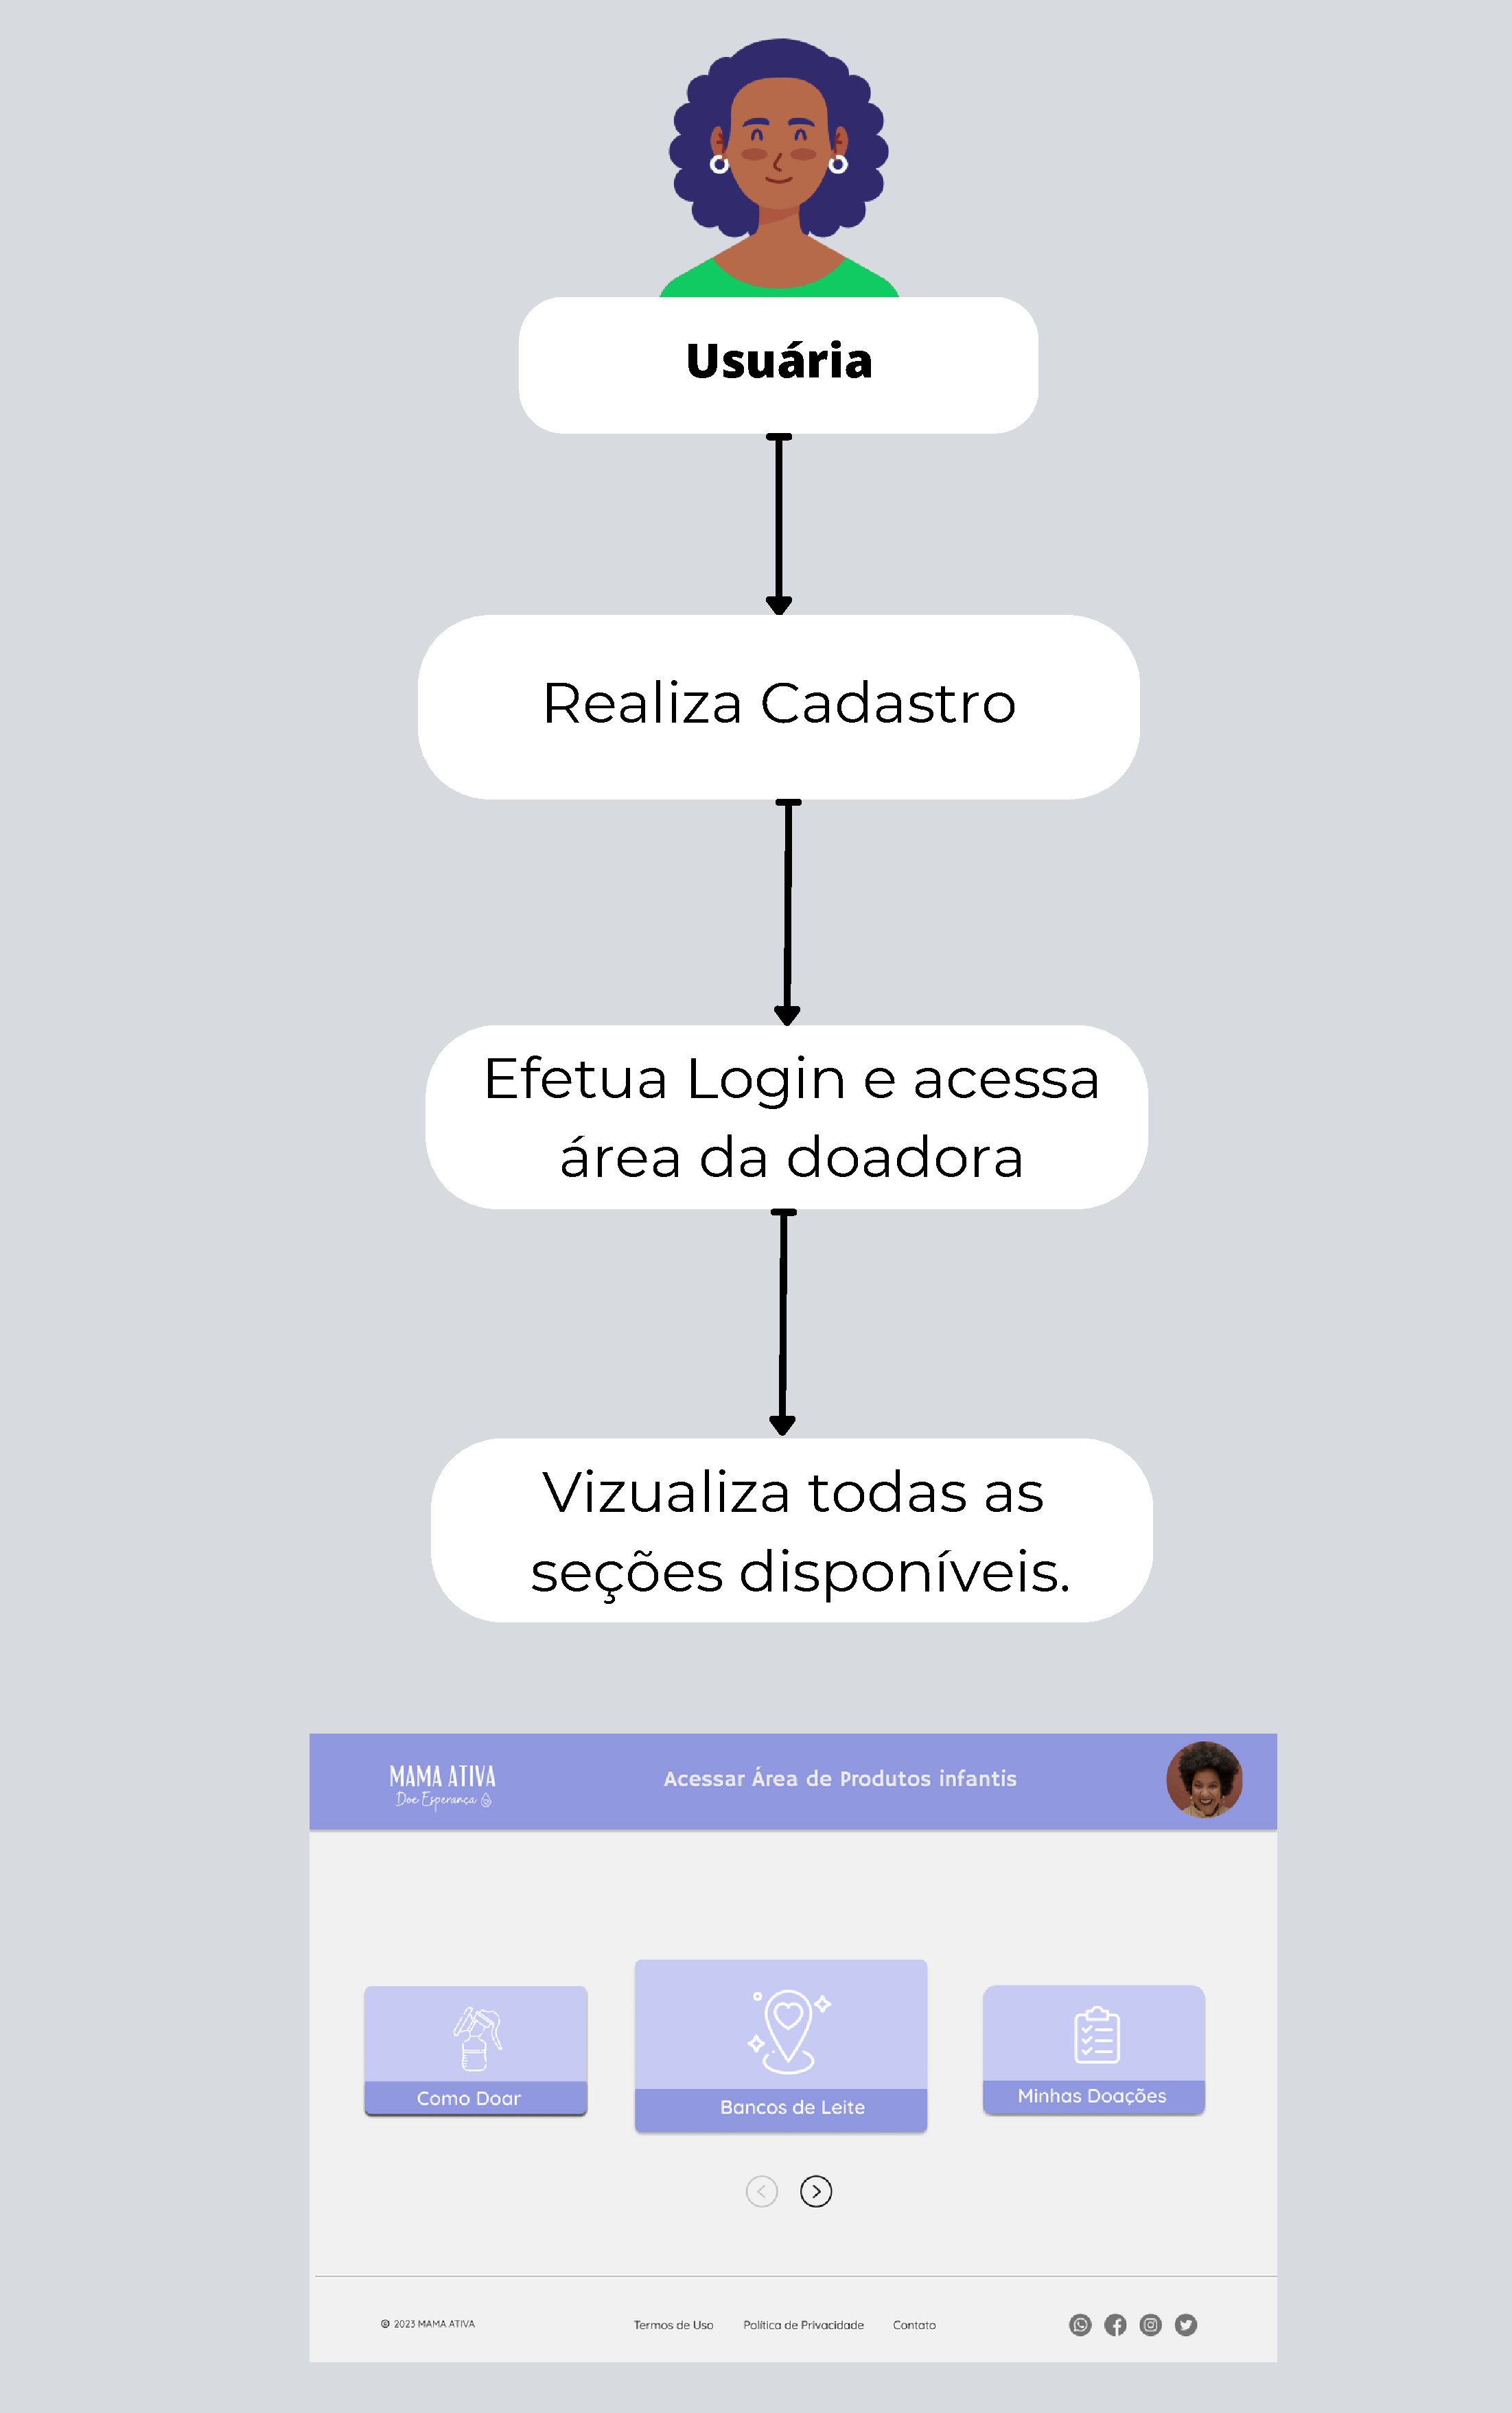
\includegraphics[width=0.45\textwidth]{Figuras/cs1.pdf}
    \caption{Caso de Uso 1}
    \label{fig:cs1}
\end{figure} 

\section{Possíveis Casos de Uso}

\begin{figure}[h!]
    \centering
    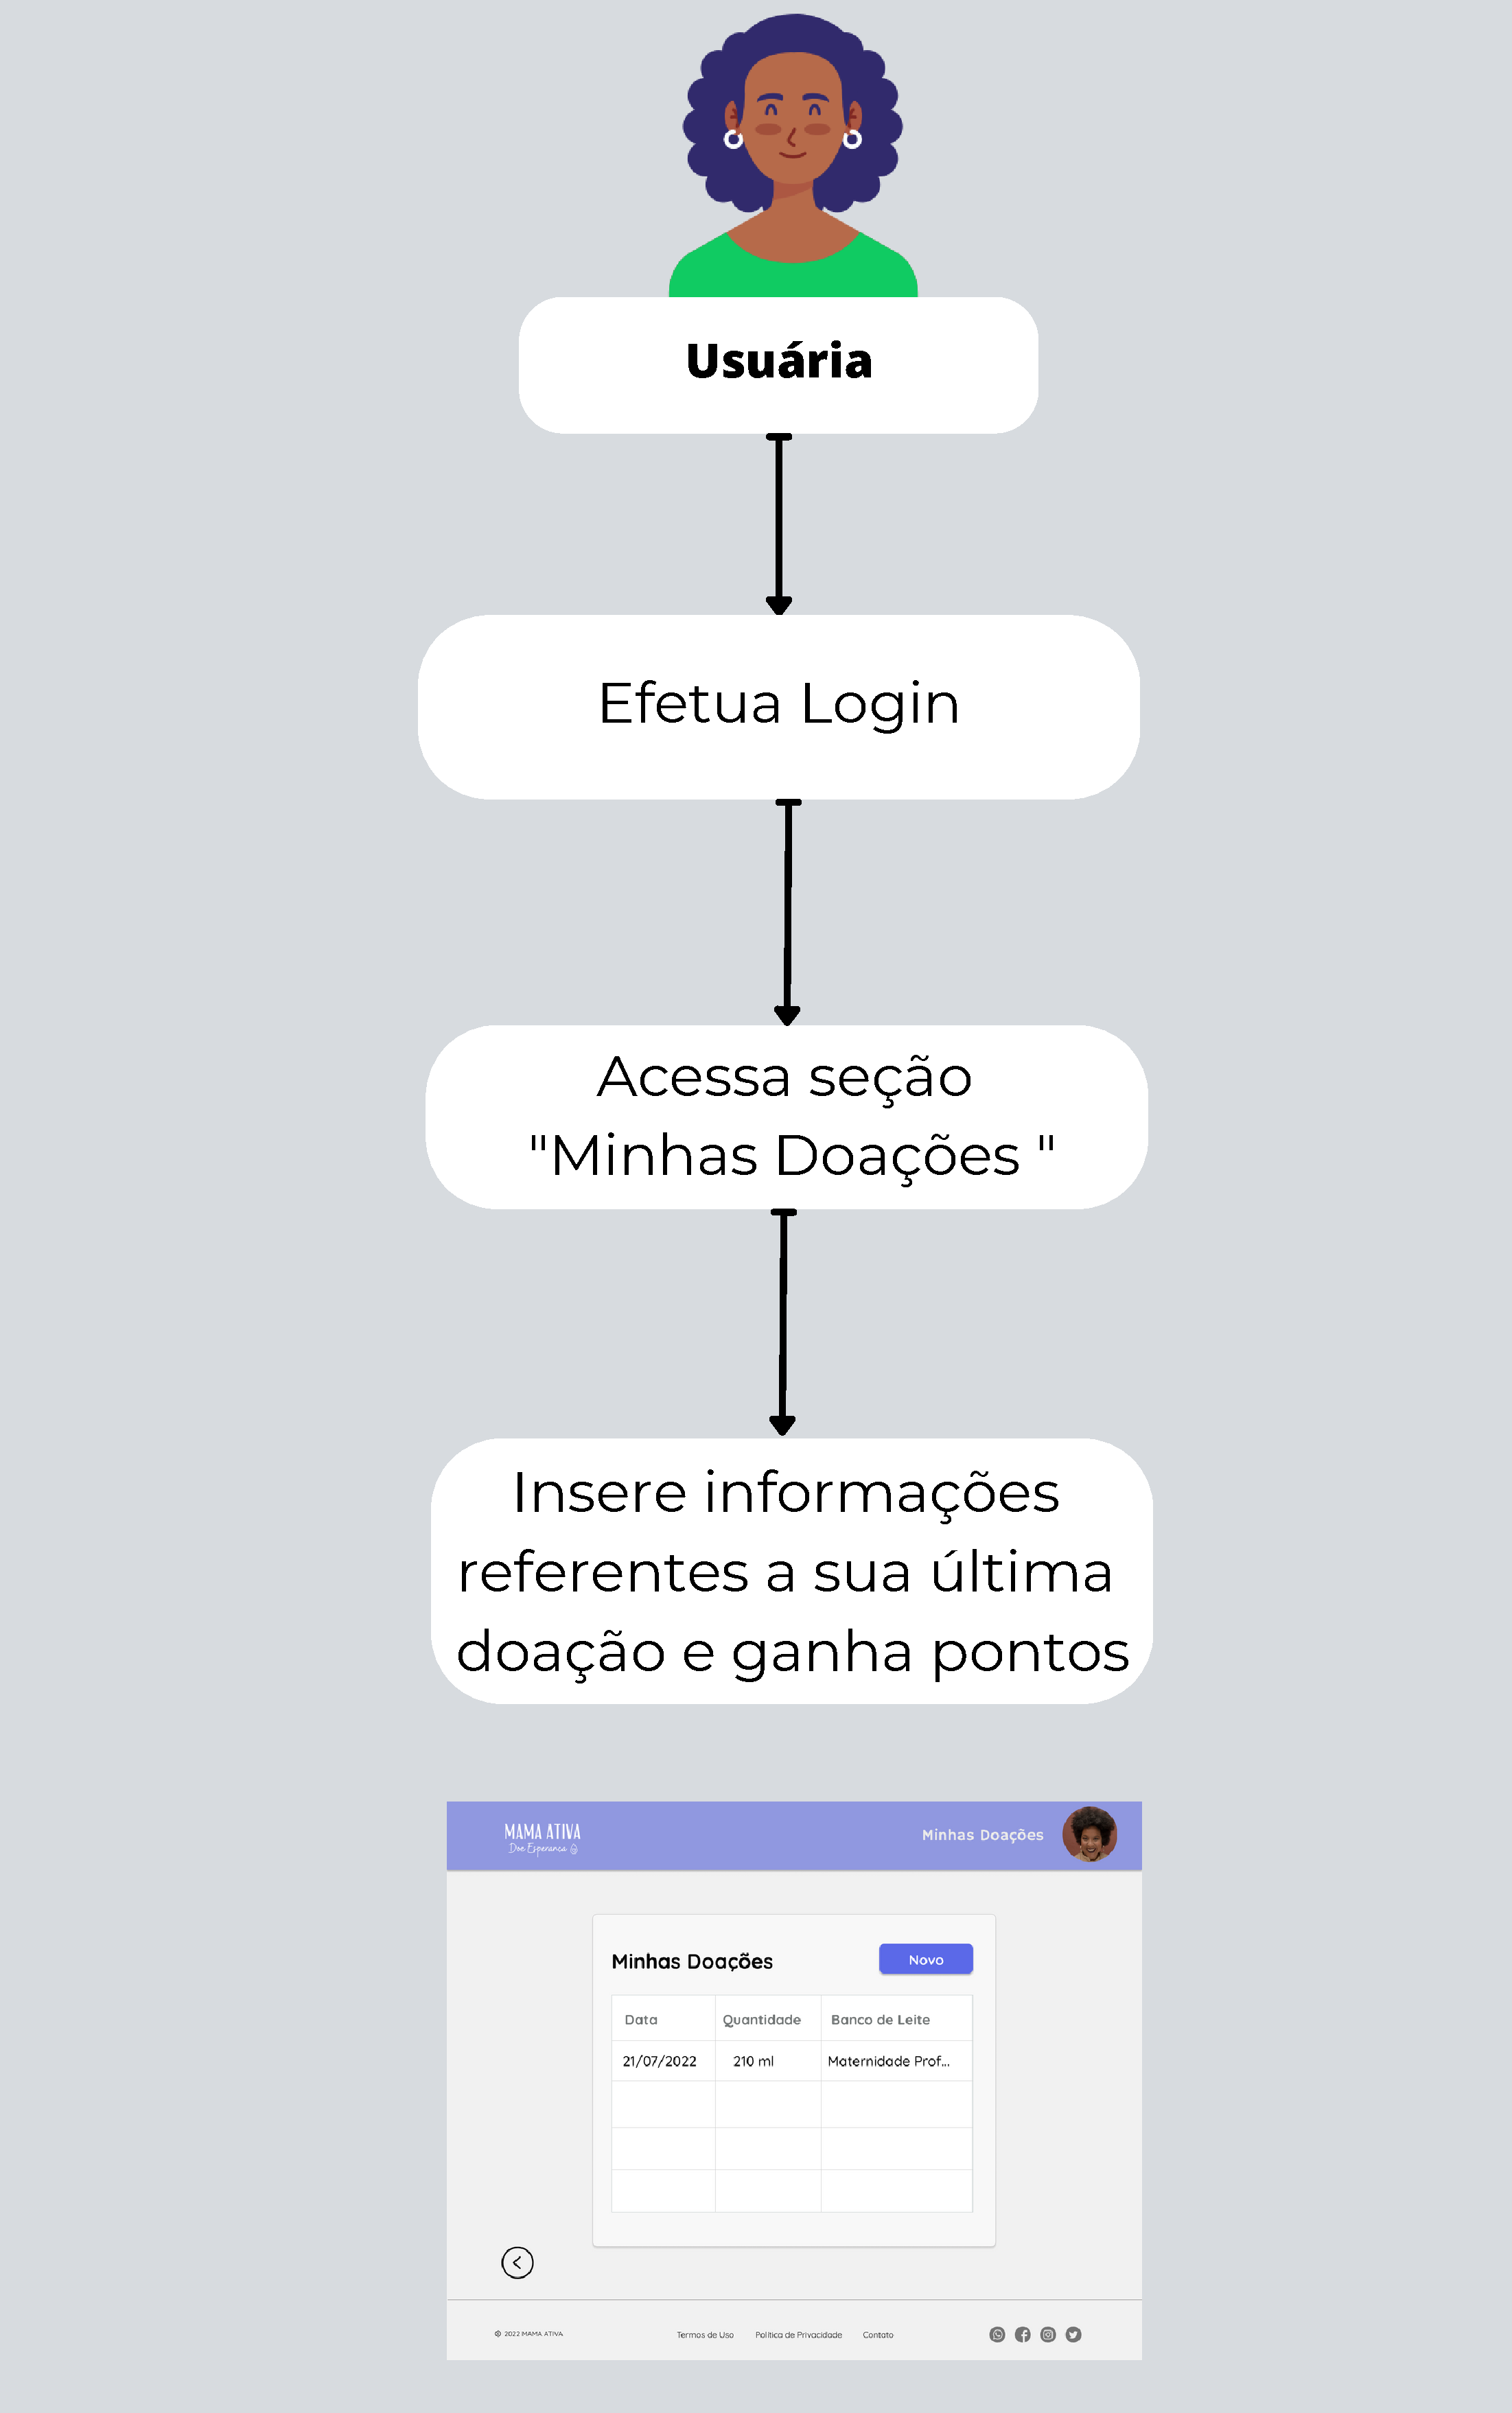
\includegraphics[width=0.45\textwidth]{Figuras/cs2.pdf}
    \caption{Caso de Uso 2}
    \label{fig:cs2}
\end{figure}

\subsection{Caso de Uso 1}
Objetivo da usuária: Realizar Cadastro e conseguir acessar área da doadora para então visualizar as seções disponíveis.

Como apresentado na Figura \ref{fig:cs1} Após o processo de cadastro, a usuária poderá fazer o login na página inicial e então poderá acessar a área da doadora. Com o intuito de facilitar a experiência de se tornar doadora, essa parte da ferramenta irá expor de forma simples e direta todas as seções disponíveis: Como doar, Bancos de Leite, Meus Registros, Mama Mídia e Minhas Conquistas. 

\subsection{Caso de Uso 2}
Objetivo da usuária: Acessar site e inserir em seção com este fim, informações referentes a sua última doação de leite.

Como apresentado na Figura \ref{fig:cs2}, ao efetuar o login, uma das seções que a usuária terá acesso é “Minhas Doações”. Aqui, a doadora poderá registrar informações relacionadas a sua última doação, como a data e a quantidade de leite doado e a unidade para qual doou. Com os dados inseridos, o aplicativo então irá fornecer pontos de acordo com a quantidade de leite doado.

\subsection{Caso de Uso 3}
Objetivo da usuária: Acessar site e a partir de seção que lista todos os Bancos de leite da cidade, encontrar o que fica mais próximo a sua casa.

Após o processo de login, a usuária poderá conferir informações sobre os bancos de leite da região metropolitana do Recife através da seção “Bancos de Leite”, como apresentado na Figura \ref{fig:cs3}. A nutriz poderá utilizar a ferramenta de busca para filtrar os bancos de acordo com o bairro e encontrar o mais próximo de sua moradia. Com o banco selecionado, é possível conferir todas as informações a respeito do local.
\begin{figure}[h]
    \centering
    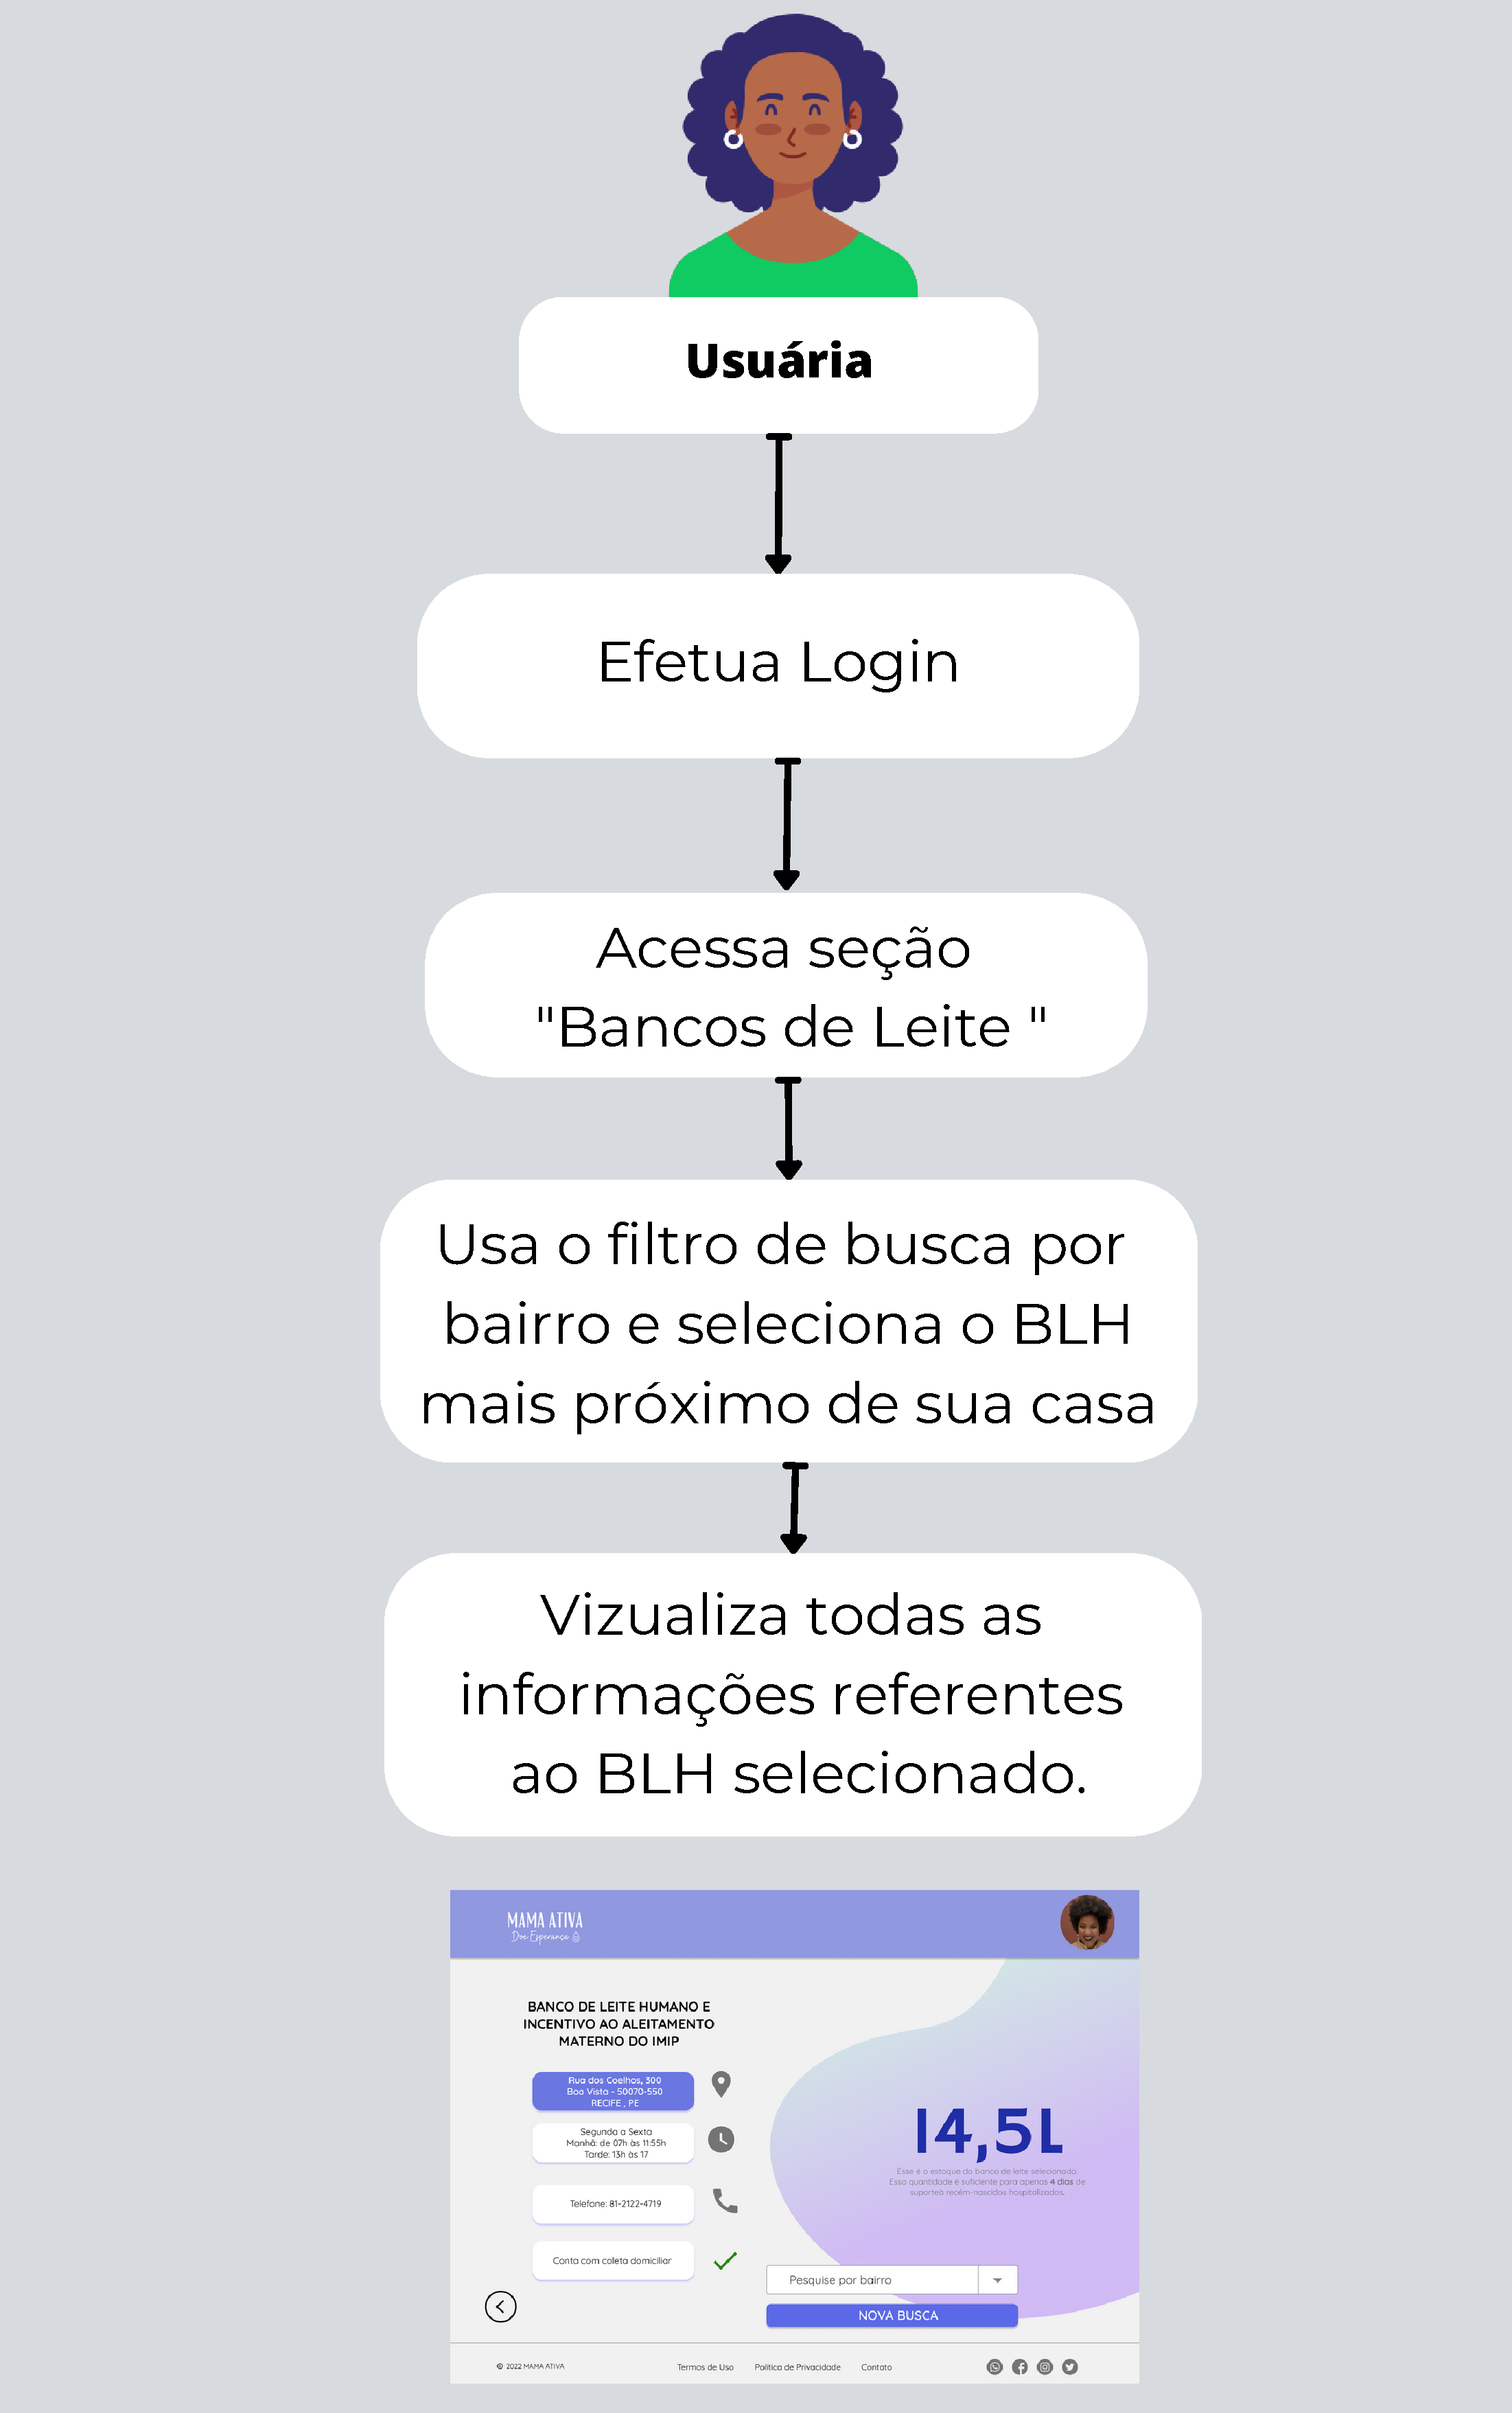
\includegraphics[width=0.45\textwidth]{Figuras/cs3.pdf}
    \caption{Caso de Uso 3}
    \label{fig:cs3}
\end{figure}


\chapter{Diagrama de Classes}


\section{Descrição do Diagrama}

O Brasil é considerado mundialmente modelo de referência em doação de leite materno, isso porque conta com a Rede de Bancos de Leite Humano (rBLH-BR), uma ação estratégica de promoção, proteção e apoio ao aleitamento materno. A iniciativa engloba ações como coleta, processamento e distribuição de leite humano para bebês prematuros ou de baixo peso que não podem ser alimentados pelas próprias mães. Em todo o país são 224 bancos de leite humano(BLH) e 216 postos de coleta, presentes em todos os estados do país.
Mesmo com uma rede tão ampla, a doação ainda não atende plenamente à demanda existente. Segundo matéria publica no Portal da Secretaria de Atenção a Saúde Primária e dados do ministério da saúde \cite{SAPS}, no ano de 2021, foram distribuídos 168 mil litros de leite humano, beneficiando 237 mil recém-nascidos. No entanto, essa quantidade representa apenas 55\% da necessidade real no país.

Um dos grandes obstáculos enfrentados no fluxo da doação de leite humano é o acesso a informação. Estudos apontam que a maioria das mulheres não tem o conhecimento de como doar, não sabem sobre a possibilidade do BLH buscar sua doação em sua casa e tampouco tem a dimensão do quanto seu gesto poderia impactar positivamente a vida de recém nascidos internados em unidades hospitalares. Trazer informação e conscientização para essas mulheres é parte da missão do Mama Ativa.

\section{Elementos do Diagrama}
No Brasil, cerca de 330 mil crianças nascidas a cada ano são prematuras ou têm baixo peso e precisam da doação de leite materno para sobreviver. O número representa 11 por cento do total de crianças nascidas no país, média de 3 milhões por ano.\cite{SAPS}
Atualmente, na cidade do Recife, são realizadas campanhas anuais de incentivo a amamentação. Porém, todos os anos, durante todo o ano, o problema se repete. Segundo \cite{FolhadePernambuco} os baixos estoques de determinados bancos chegaram recentemente a níveis preocupantes. Outra combinação preocupante que identificamos a partir de dados fornecidos pela \cite{RedeBLH}, foi que a situação dos estoques piora em datas festivas, como carnaval, natal e réveillon, ao mesmo tempo em que a necessidade deste alimento para os recém-nascidos internados em UTIs aumenta.
Identificado este problema e nos aprofundando mais em pesquisas sobre o tema, constatamos que não existe hoje, no Recife, nenhuma plataforma tecnológica que atenda a essa demanda. Dito isto, propomos a criação de uma aplicação que propõe, através de uma experiência atraente, divertida e "gameficada", incentivar o aumento de doações de leite humano(LH) em nosso estado.

Com o objetivo de entender melhor os fatores que estão diretamente relacionados a doação de leite humano, realizamos uma revisão de literatura acerca do tema. Analisamos 10 artigos científicos além de sites institucionais e governamentais. Foi observado que as principais razões encontradas para a doação de LH não começam no propósito da doação em si. Diversos artigos apontam que a maioria das mulheres procuraram os BLHs das suas cidades buscando orientação para a amamentação. Essas, relatam que após o primeiro contato com profissionais das unidades passam a saber da possibilidade do armazenamento e da doação do seu leite. 

Outras razões apontadas como relevantes para que a doação não aconteça seriam: falta de suporte emocional, ausência de rede de apoio, falta de conhecimento e dificuldade em encontrar informações acerca do fluxo de doação de LH.

Os BLHs possuem um controle de armazenamento sobre as doações que são recebidas e a quantidade disponível para doação. Antes do alimento ser direcionado para o consumo, ele passa por um processo de pasteurização, que consiste em aquecê-lo a uma temperatura elevada por um período determinado, com o objetivo de inativar 100\% dos microorganismos patogênicos, que são aqueles capazes de causar doenças em seres humanos, e cerca de 99,99\% da microbiota saprófita, que são microorganismos que auxiliam na decomposição de matéria orgânica morta. O problema é que, segundo \cite{RedeBLH}, nesse processo aproximadamente 30\% do leite doado é desperdiçado devido principalmente à forma inadequada de coleta e armazenamento. Muitas mães utilizam recipientes com tampas de alumínio, tornando-os inutilizáveis para doações posteriores. Além disso, é comum que o leite seja entregue contaminado por sujeira ou danificado pelo congelamento.

Em resumo, os principais problemas encontrados consistem de: 
\begin{itemize}
    \item Falta de acesso a informação
    \item Ausência de uma solução efetiva e durável no estímulo a doação de leite
\end{itemize} 

\section{Relações entre as classes}

\subsection{Notas e Observaçôes}

\begin{itemize}
  \item Conscientizar nutrizes acerca da importância e dos benefícios da doação do leito materno.
  \item Disponibilizar o quantitativo dos estoques dos BLH atualizados semanalmente, para que as doadoras tenham ciência das unidades com maior necessidade e assim possam direcionar melhor sua doação.
  \item "Gameficar" a aplicação a fim de promover um maior engajamento por parte dos usuários.
\end{itemize}


